\chapter{Những công trình liên quan}
Hai công trình được công bố công khai có đề tài tương đồng với đề tài luận văn này đó là 
``Automated Bitcoin Trading via Machine Learning Algorithms'' \cite{AutomatedBitcoinTrading}
và ``Predicting the price of Bitcoin using Machine Learning'' \cite{PredictingThePriceOfBitcoin}.
Đây là hai công trình sử dụng trực tiếp Máy học trong bài toán dự đoán xu hướng 
giá trị BTC, mỗi công trình đều có một hướng tiếp cận riêng biệt và đồng thời 
cũng cho ra các kết quả khác nhau.\\\\
Trong bài báo \cite{AutomatedBitcoinTrading}, nhóm tác giả sử dụng một tập dữ 
liệu về giá trị BTC, tập dữ liệu này chứa khoảng 120.000 mẫu được thu thập thông 
qua API của Coinbase và OKCoin (đây là những loại ví điện tử được dùng để lưu 
trữ và trao đổi BTC, Coinbase xây dựng ở San Francisco và OKCoin xây dựng ở Bắc 
Kinh) - gọi đây là tập dữ liệu thứ nhất. Ngoài ra, nhóm tác giả còn thu thập 
thêm tập dữ liệu giá thường nhật kèm theo các thông tin về mạng Bitcoin, tập dữ 
liệu này bao gồm 26 đặc trưng nhưng chỉ được dùng 16 đặc trưng cho quá trình 
phân tích và chạy giải thuật - gọi đây là tập dữ liệu thứ hai.\\\\
Với tập dữ liệu thứ nhất, nhóm tác giả tiếp cận vấn đề bằng phương pháp chuỗi 
thời gian (Time Series) với 2 khoảng thang thời gian là 10 giây và 10 phút. Còn 
lại, tập dữ liệu thứ hai được sử dụng như một tập dữ liệu phân lớp đơn thuần.
Kết quả chi tiết của các giải thuật LR, SVM và RF:
\begin{table}[h]
\centering
\begin{tabular}{ |c|c|c|c| }
\hline
Tham số đánh giá & 10 giây - LR & 10 phút - SVM & 10 phút - RF \\
\hline
Recall & 54.29\% & 52.40\% & 54.00\% \\
\hline
Specificity & 57.70\% & 57.60\% & 61.90\% \\
\hline
Precision & 57.40\% & 55.10\% & 58.10\% \\
\hline
Accuracy & 8.50\% & 53.90\% & 57.40\% \\
\hline
\end{tabular}
\caption{Bảng đánh giá với tập dữ liệu thứ nhất}
\end{table}\\
Lưu ý, nhóm tác giả ký hiệu giải thuật LR là Binomial GLM và tham số đánh giá 
Recall là Sensitivity.
\begin{table}[h]
\centering
\begin{tabular}{ |c|c|c|c| }
\hline
Tham số đánh giá & LR & SVM & RF \\
\hline
Recall & 97.90\% & 3.48\% & 100\% \\
\hline
Specificity & 99.39\% & 55.14\% & 93.92\% \\
\hline
Precision & 97.90\% & 8.39\% & 77.62\% \\
\hline
Accuracy & 98.79\% & 27.16\% & 94.98\% \\
\hline
\end{tabular}
\caption{Bảng đánh giá với tập dữ liệu thứ hai}
\end{table}\\
Với công trình nghiên cứu \cite{PredictingThePriceOfBitcoin}, tác giả sử dụng 
một hướng tiếp cận khác hơn so với bài báo \cite{AutomatedBitcoinTrading}. Với 
tập dữ liệu giá BTC được thu thập thông qua CoinDesk từ ngày 19/8/2013 đến ngày 
19/07/2016, tác giả sử dụng các kiến thức về Học sâu (Deep Learning) như là một 
công cụ chính để phân tích và giải quyết bài toán. Ngoài ra, trong công trình 
này còn nhắc đến việc sử dụng mô hình ARIMA - một dạng mô hình phân tích chuỗi 
thời gian - như là một giải thuật dùng để so sánh với giải thuật chính. Giải 
thích quyết định này, tác giả đã đưa ra lý luận phân tích rằng, ARIMA mặc dù là 
một mô hình dữ đoán chuỗi thời gian phổ biến, tuy nhiên, mô hình này lại phụ 
thuộc vào giả định tập dữ liệu là tuyến tính về thời gian và điều này không phù 
hợp với tập dữ liệu đang được sử dụng - tập dữ liệu được sử dụng là phi tuyến 
tính.\\\\
Đi vào chi tiết, giải thuật học sâu được sử dụng đó là RNN một dạng của 
mạng neural (xem phần 3.3.3), RNN có khả năng sử dụng cả hai giải thuật lan 
truyền là lan truyền thuận và lan truyền ngược. Ngoài ra, tác giả còn sử dụng 
một biến thể khác của RNN, đó là LSTM, ở RNN các tham số mạng được tìm bằng 
giải thuật di truyền (Genetic Algorithm), khác với LSTM sử dụng giải thuật tối 
ưu Bayesian (Bayesian Optimisation) để tìm tham số mạng. Kết quả của quá trình 
chạy giải thuật:
\begin{table}[h]
\centering
\begin{tabular}{ |c|c|c|c| }
\hline
Tham số đánh giá & LSTM & RNN & ARIMA \\
\hline
Recall & 37.00\% & 40.40\% & 14.7\% \\
\hline
Specificity & 61.30\% & 56.65\% & 100\% \\
\hline
Precision & 35.50\% & 39.08\% & 100\% \\
\hline
Accuracy & 52.78\% & 50.25\% & 50.05\% \\
\hline
\end{tabular}
\caption{Bảng đánh giá các giải thuật học sâu và ARIMA}
\end{table}\\
Ngoài hai công trình trên, chúng ta sẽ tiếp tục tham khảo các vấn đề liên quan 
khác như là dự đoán xu hướng giá trị vàng và dự đoán xu hướng giá trị cổ phiếu.
Mặc dù các công trình này không đi giải quyết vấn đề dự đoán giá trị BTC, nhưng 
với cách nhìn tổng quát, vấn đề chung vẫn là sử dụng Máy học để dự đoán giá trị 
các tài sản giao dịch. Vàng, cổ phiếu là hai tài sản giao dịch đặc trưng và lâu 
đời, vì thế các vấn đề về dự đoán của hai tài sản giao dịch này cũng đã được 
khai thác và phát triển từ lâu. Hai công trình cụ thể được tham khảo trong luận văn là: 
``Predicting Gold Prices'' \cite{PredictingGoldPrices} và 
``Machine Learning in Stock Price Trend Forecasting'' 
\cite{StockPriceTrendForecasting} \\\\ 
Bài báo \cite{PredictingGoldPrices} liên quan đến ứng dụng Máy học cho việc dự đoán 
giá vàng, tác giả đã chọn hướng tiếp cận học có giám sát và cụ thể là bài toán 
phân lớp. Tập dữ liệu mà tác giả sử dụng là tập dữ liệu giá vàng từ đầu năm 2007 
đến cuối năm 2013 với khoảng 1700 mẫu và được lấy từ trang web của USA Gold, 
đồng thời sử dụng hai giải thuật phân lớp là SVM và LR.
Trong đó, khi gặp phải vấn đề mất cân đối trong tập dữ liệu (nhãn $positive$ 
lớn hơn rất nhiều sao với nhãn $negative$) tác giả đã sử dụng giải thuật SVM 
với nhiều lần điều chỉnh mô hình như: sử dụng kernel RBF, sử dụng kernel tuyến 
tính với L1,... nhưng đều cho ra kết quả thấp (Accuracy nằm trong khoảng 50\% 
- 51\%). Với kết quả như vậy, tác giả đã quyết định sử dụng SVM như một giải 
thuật dùng để so sánh và đánh giá với giải thuật còn lại. Với một hướng tiếp 
cận khác, LR được sử dụng để giải quyết bài toán, kết quả được ghi nhận như 
bảng sau.
\begin{table}[h]
\centering
\begin{tabular}{ |c|c| }
\hline
Precision & 69.90\% \\
\hline
Recall & 72.31\% \\
\hline
Accuracy & 69.30\% \\
\hline
\end{tabular}
\caption{Bảng đánh giá giải thuật LR}
\end{table}\\
Với kết quả trên, các tham số đánh giá cho kết quả trong khoảng gần bằng 70\% 
và tác giả xem đây là một kết quả có ý nghĩa.\\\\
Bài báo \cite{StockPriceTrendForecasting} liên quan đến ứng dụng Máy học cho việc 
dự đoán giá trị cổ phiếu (cụ thể là công ty 3M), nguồn dữ liệu được sử dụng là 
Bloomberg Data Terminal với khoảng 1400 mẫu. Nhóm tác giả đã sử dụng bốn 
giải thuật trong quá trình phân tích và giải quyết bài toán đó là: GDA, LR, SVM, 
QDA.\\\\
Ngoài ra, để có thể tìm ra một hướng giải quyết tối ưu, nhóm tác giả tiếp cận 
vấn đề dựa trên hai mô hình khác nhau. Thứ nhất, mô hình Ngày tiếp theo (Next-Day 
Model) với mục tiêu đi dự đoán xu hướng giá trị của cổ phiếu trong ngày tiếp 
theo. Và thứ hai, mô hình Dài hạn (Long-Term Model) với mục tiêu đi dự đoán xu 
hướng giá trị của $n$ ngày tiếp theo.\\\\
Kết quả đánh giá của 4 giải thuật cho mô hình Ngày tiếp theo:
\begin{table}[h]
\centering
\begin{tabular}{ |c|c|c|c|c| }
\hline
Model & LR & GDA & QDA & SVM \\
\hline
Accuracy & 44.5\% & 46.4\% & 58.2\% & 55.2\% \\
\hline
\end{tabular}
\caption{Bảng đánh giá mô hình Ngày tiếp theo }
\end{table}\\
Đồ thị đánh giá của 4 giải thuật cho mô hình Dài hạn:
\begin{figure}[h!]
\centering
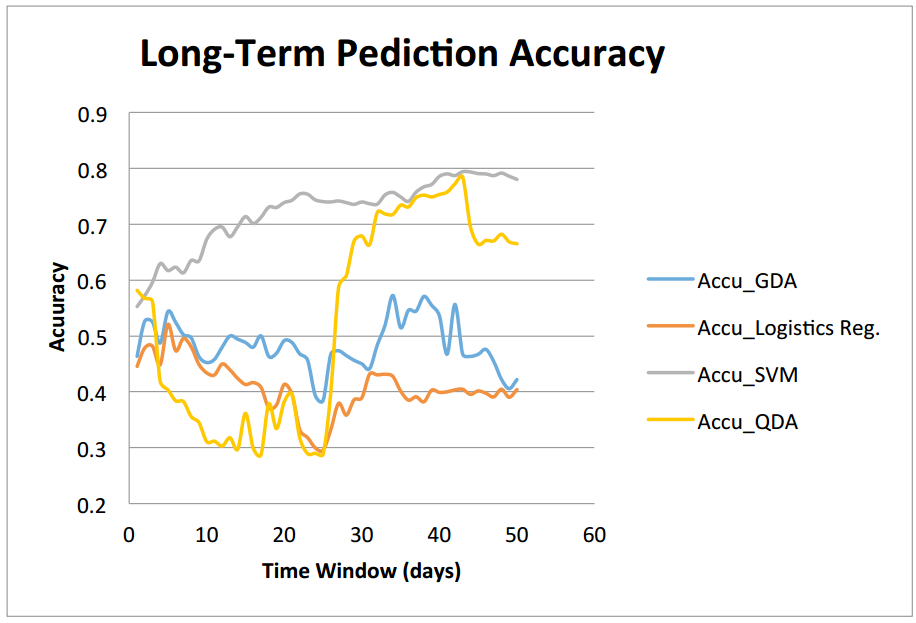
\includegraphics[height=3.5in, keepaspectratio=true]{longtermmodel.png}
\caption{Đồ thị đánh giá mô hình Dài hạn}
\end{figure}\\
Hai mô hình với hai kết quả, ta thấy ở mô hình Dài hạn hai giải thuật SVM và 
QDA cho kết quả Accuracy gần bằng 80\% với $n=44$ ngày, so sánh với mô hình 
Ngày tiếp theo Accuracy gần bằng 60\% ta có thể thấy mô hình dài hạn cho kết 
quả có ý nghĩa hơn. Nhưng một hạn chế rất lớn của công trình này, nhóm tác giả 
chỉ sử dụng một tham số đánh giá duy nhất là Accuracy mà bỏ qua Precision và 
Recall. Việc đánh giá chỉ dựa trên duy nhất một tham số sẽ không thể tổng quát 
được kết quả đầu ra, vì vậy mà dẫn đến nguy cơ không phát hiện các vấn đề về 
lệch dữ liệu hoặc overfitting.\\\\ 
Tổng quan qua các công trình trên và tham khảo một số công trình khác, nhận thấy 
đa số các hướng tiếp cận đều đi theo một phương pháp tổng quát chung, nó bao gồm các bước 
cơ bản như:
\begin{enumerate}
\item Xây dựng không gian vector đặc trưng phù hợp với tính chất bài toán
\item Lựa chọn mô hình phân tích
\item Sử dụng các giải thuật phân lớp điển hình trong Máy học như là 
SVM, LR ...
\item Đánh giá giải thuật bằng các tham số Accuracy, Recall, Precision.
\end{enumerate}
Từ những đục kết trên, bản thân nhận thấy các bước trên cũng chính là phương pháp 
nên dùng để tiếp cận đề tài. Ngoài ra, nhận thấy ở hai công trình trên chưa đề 
cập đến việc sử dụng một giải thuật rất được phổ biến hiện nay, nó nổi lên như 
một đại diện của Học sâu đó là MNN. Do đó mà luận văn này sẽ sử dụng MNN như là 
một giải thuật bổ sung trong quá trình so sánh và đánh giá so với các giải thuật 
phân lớp khác.